% Generated 2021-02-06 01:28:14 +0530
\subsection{SolidModel} \label{sec:SolidModel}


A \block{SolidModel} is a \block{Configuration} that references a file with the three-dimensional geometry of the \block{Component} or \block{Composition}. The geometry \textbf{MAY} have a transformation and a scale to position the \block{Component} with respect to the other \block{Component}s. A geometry file can contain a set of assembled items, in this case, the \block{SolidModel} reference the \property{id}[SolidModel] of the assembly model file and the specific item within that file.

The \block{SolidModel} \textbf{MAY} provide a translation, rotation, and scale to correctly place it relative to the other geometries in the machine. If the \block{Component} can move and has a \block{Motion} \block{Configuration}, the \block{SolidModel} will move when the \block{Component} or \block{Composition} moves.

Either an \property{href}[SolidModel] or a \property{modelIdRef}[SolidModel] and an \property{itemRef}[SolidModel] \textbf{MUST} be specified.

\begin{figure}[ht]
  \centering
    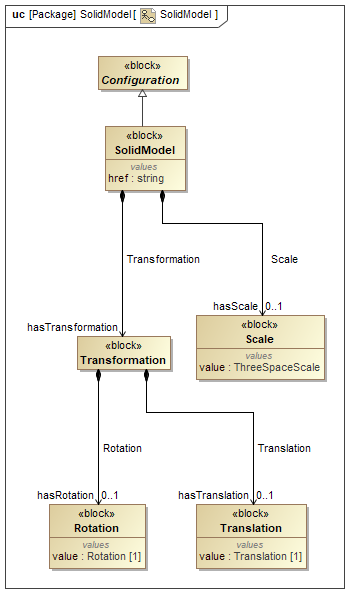
\includegraphics[width=1.0\textwidth]{figures/SolidModel.png}
  \caption{SolidModel Diagram}
  \label{fig:SolidModel Diagram}
\end{figure}

\FloatBarrier


Note: See \fig{SolidModel Schema Diagram} for XML schema.


\subsubsection{SolidModel}




\block{SolidModel} is a \block{Configuration} that references a file with the three-dimensional geometry of the \block{Component} or \block{Composition}.


\paragraph{Attributes of SolidModel}\mbox{}
\label{sec:Attributes of SolidModel}

\tbl{Attributes of SolidModel} lists the attributes of \texttt{SolidModel}.

\begin{table}[ht]
\centering 
  \caption{Attributes of SolidModel}
  \label{table:Attributes of SolidModel}
\tabulinesep=3pt
\begin{tabu} to 6in {|l|l|l|} \everyrow{\hline}
\hline
\rowfont\bfseries {Attribute} & {Type} & {Multiplicity} \\
\tabucline[1.5pt]{}

\property{id}[SolidModel] & \texttt{ID} & 1 \\
\property{solidModelIdRef}[SolidModel] & \texttt{IDREF} & 0..1 \\
\property{mediaType}[SolidModel] & \texttt{MediaTypeEnum} & 1 \\
\property{coordinateSystemIdRef}[SolidModel] & \texttt{IDREF} & 0..1 \\
\end{tabu}
\end{table}
\FloatBarrier

Descriptions for attributes of \block{SolidModel}:

\begin{itemize}

\item \property{id}[SolidModel] \newline The unique identifier for this entity within the \block{MTConnectDevices} document.

\item \property{solidModelIdRef}[SolidModel] \newline The associated model file if an item reference is used.

\item \property{mediaType}[SolidModel] \newline The format of the referenced document.

\texttt{MediaTypeEnum} Enumeration:

\begin{itemize}
\item \texttt{STEP} \newline ISO 10303 STEP AP203 or AP242 format. 
\item \texttt{STL} \newline Stereolithography file format. 
\item \texttt{GDML} \newline Geometry Description Markup Language. 
\item \texttt{OBJ} \newline Wavefront OBJ file format.
 
\item \texttt{COLLADA} \newline ISO 17506. 
\item \texttt{IGES} \newline Initial Graphics Exchange Specification. 
\item \texttt{3DS} \newline Autodesk file format. 
\item \texttt{ACIS} \newline Dassault file format. 
\item \texttt{X\textunderscore T} \newline Parasolid XT Siemens data interchange format. 
\end{itemize}


\item \property{coordinateSystemIdRef}[SolidModel] \newline A reference to the coordinate system for this \block{SolidModel}.

\end{itemize}


\paragraph{Elements of SolidModel}\mbox{}
\label{sec:Elements of SolidModel}

\tbl{Elements of SolidModel} lists the elements of \texttt{SolidModel}.

\begin{table}[ht]
\centering 
  \caption{Elements of SolidModel}
  \label{table:Elements of SolidModel}
\tabulinesep=3pt
\begin{tabu} to 6in {|l|l|} \everyrow{\hline}
\hline
\rowfont\bfseries {Element} & {Multiplicity} \\
\tabucline[1.5pt]{}
\texttt{Transformation} & 1 \\
\texttt{Scale} & 0..1 \\
\end{tabu}
\end{table}
\FloatBarrier


Descriptions for elements of \block{SolidModel}:

\begin{itemize}

\item \block{Transformation} \newline The translation of the origin to the position and orientation.

At a minimum, a \block{Translation} or \block{Rotation} \textbf{MUST} be given.

\item \block{Scale} \newline The \block{SolidModel} \block{Scale} is either a single multiplier applied to all three dimensions or a three space multiplier given in the X, Y, and Z dimensions in the coordinate system used for the \block{SolidModel}.
\end{itemize}



\subsubsection{Scale}
\label{sec:Scale}



The \block{SolidModel} \block{Scale} is either a single multiplier applied to all three dimensions or a three space multiplier given in the X, Y, and Z dimensions in the coordinate system used for the \block{SolidModel}.


The value of \texttt{Scale} \MUST be \texttt{ThreeSpaceScale}.


